\documentclass{article}
\usepackage{amsmath}
\usepackage{amssymb}
\usepackage{graphicx}
\usepackage{enumitem}
\usepackage[utf8]{inputenc}
\graphicspath{{/home/stephanie/Escritorio/THC/Taller-de-Herramientas-Computacionales/Clases/Latex/Imagenes/}}

\title{\Huge Taller de Herramientas Computacionales}
\author{Stephanie Escobar Sánchez}
\date{15/enero/2019}
\begin{document}
	\maketitle
\begin{center}
	
\includegraphics[scale=0.40]{1.png}	
\end{center}
\newpage
\title{\Huge Bitácora clase 6} \\
\\
La clase comenzó viendo las diferencias entre virtualización y emulación, debido a que no todos tienen una maquina con sistema operativo linux y optaron por una máquina virtual. Una máquina virtual es más rápida que un emulador debido a que un emulador solo imita lso procesos pero en una maquina virtual es posible incluso instalar programas del sistema operativo que se virtualiza.\\
Otro concepto que vimos fue de bios, que es una memoria que contiene la informacion de la computadora: Procesador, memoria, características específicas del equipo.\\
\\
Hablamos sobre las distintas distribuciones de Linux adaptadas a necesidades específicas y tipo de computadora, las distribuciones tienen distintas versiones llamadas flavors y algunas de ellas son más ligeras que otras, lo cual permite que corran más rápido en computadoras con menor capacidad. El comando \$ top permite ver los núcleos de la computadora para ver la capacidad que tiene y decidir el sistema operativo. Nosotros utilizamos ubuntu y fedora por la cantidad de funciones que tienen y porque son sistemas fáciles de instala.\\
\\
Un algoritmo es un proceso de instrucciones finitas, en la clase aprendimos a hacer algoritmos. Primero planteando un problema y pensar en la solución de forma teórica. El problema de la clase fue ¿Cómo se define la raíz cuadrada? teníamos que crear una función que nos regresara la raíz cuadrada de un número para ello necesitábamos llegar a una aproximación debido a que la computadora no tiene a todos los números reales, por lo que hay un número mínimo que puede darnos.
Pensamos el problema a partir de un cuadrado, sabemos que un cuadrado con lado $\sqrt{x}$ tendrá por área x, sabemos también que un rectángulo con lados x y 1 tiene área x. Primero debemos buscar una forma de pasar del segundo cuadrado al primero.
\begin{center}
	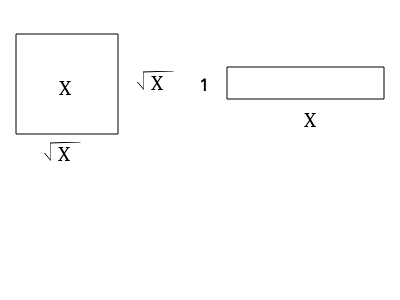
\includegraphics[scale=0.40]{2.png}	
\end{center}
Lo primero que hacemos es pensar en ir cambiando los valores a los lados hasta que su diferencia sea muy pequeña, por tanto primero hacemos un promedio muy lo llamamos h, después esa h se la restamos al otro número.\\
\\
Vimos otros conceptos y comandos de python. Una asignación consiste en asignar valores a una variable a partir de una función o directamente. Las asignaciones se hacen poniendo una letra, un signo de igual y lo que queremos guardar.
Un bloque en python es todo lo que esta indexado, todo lo que esta después de los dos puntos. En python son importantes los bloques debido a que nos permite de una forma visual anidar instrucciones y saber a que bloque corresponde un comando. Es en donde importan los espacios en python, además permiten hacer cadenas de instrucciones.\\
\\
Otra cosa importante de python es que no siempre es necesario que nos muestre el resultado de lo que hacemos, muchas veces lo queremos guardar para seguir haciendo más comandos y ocuparlo después. Pedirle al programa que lo imprima puede hacer que la computadora tarde más en correrlo, lo mejor es que el resultado se quede guardado hasta el momento en que lo necesitemos.\\
\\
Al final de la clase vimos un par de comandos que son muy importantes, el \textit{if} y el \textit{while}. El comando if es un condicional y permite poner ciertas condiciones que deberían cumplirse para que ejecute una acción, si esto no ocurre, el comando \textit{else} ejecuta otra acción con el resultado. \textit{while} es un comando que permite crear ciclos y que una acción se repita mientras ciertas condiciones se cumplan, en el momento en que la condición no se cumpla el programa se detiene. Estos dos comandos son muy importantes porque nos permiten crear programas básicos y algunos más complejos.

\end{document}
